\chapter{Vorgehen}
\label{chapter:vorgehen}
Im Folgenden wird das Vorgehen erläutert, um die im ersten Kapitel genannten Ziele zu erreichen.
Dabei wurde folgende sieben Aktivitäten ausgearbeitet, die nicht auf einander aufbauen,
sondern in einem iterativen Prozess miteinander verzahnt sind,
welcher in der Grafik \ref{img:process} veranschaulicht und im Weiteren näher erläutert wird. \\

\begin{itemize}
    \item Sichtung der Publikationen
    \item Identifizierung von Kontextfaktoren
    \item Klassifizierung von Kontextfaktoren
    \item Charaktierisierung von Publikationen
    \item Dokumentierung und Erstellung von Artefakten
    \item Analyse der Artefakte
    \item Anfertigung einer Taxonomie
\end{itemize}

\begin{figure}[thb]
    \centering
    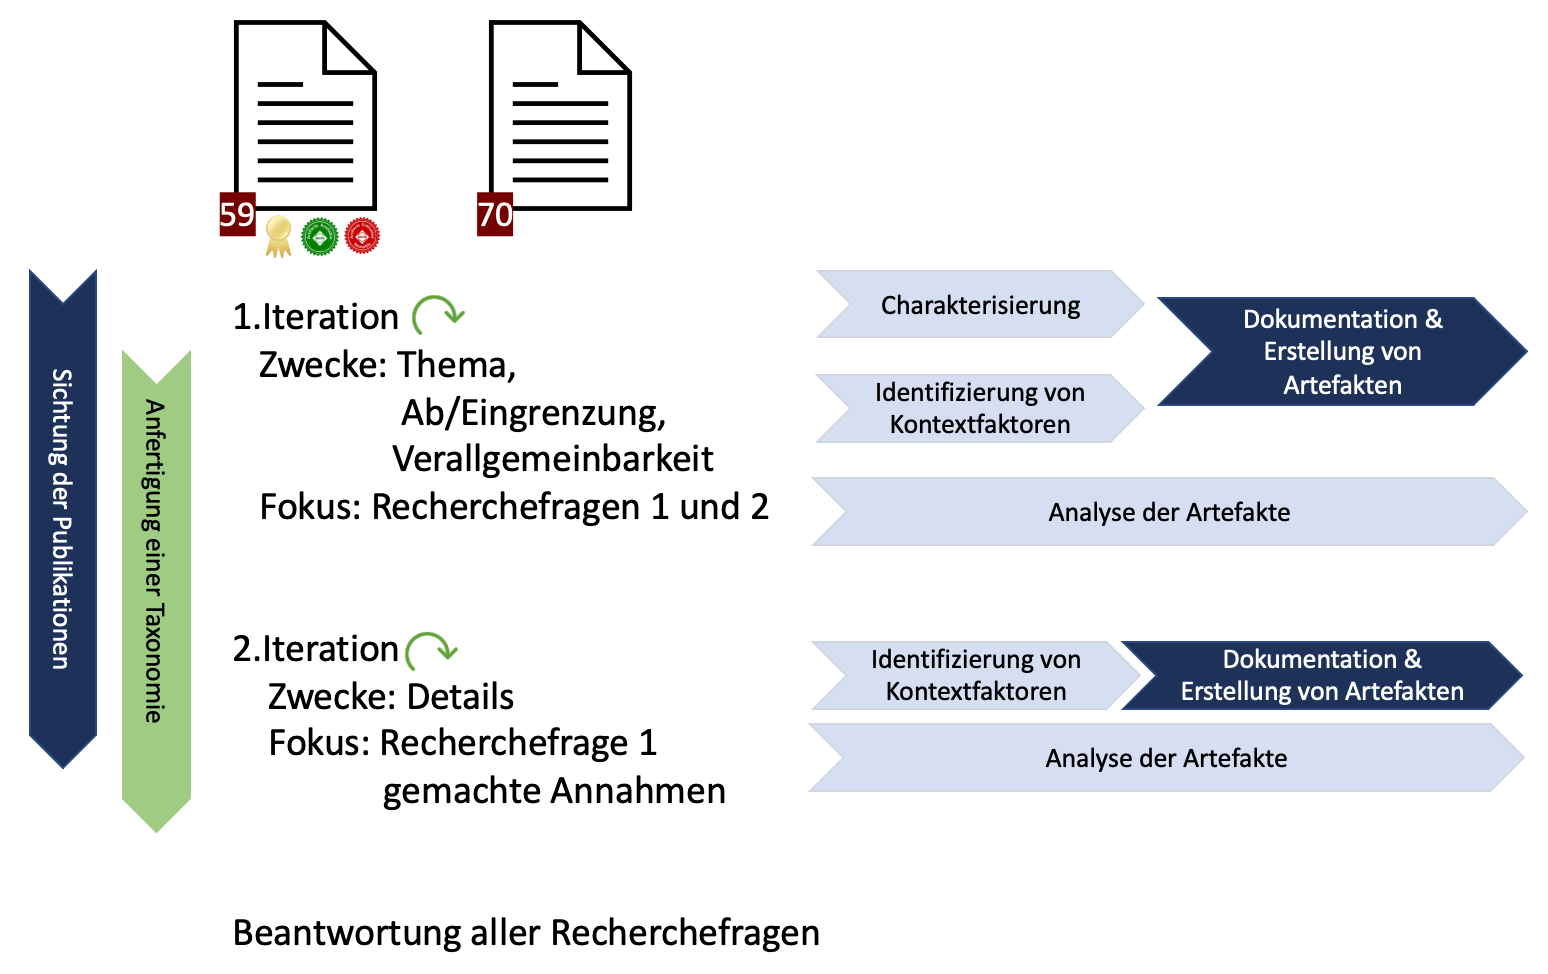
\includegraphics[clip,width=0.9\linewidth]{content/images/03-Vorgehen}
    \caption{Vorgehen}
    \label{img:process}
\end{figure}

\clearpage

\section{Sichtung der Publikationen}
Zur Identifikation von Kontextfaktoren, werden die Publikationen der technischen Artikel veröffentlicht in der ISCE 2020, in mehreren Iterationen gesichtet. \\

In der 1. Iteration basiert die Reihenfolge, anhand welcher die Publikationen gelesen werden, auf die Auszeichnungen und Badges, die die Publikationen erhalten haben, da angenommen wird, dass diese Publikationen eine höhere Qualität aufweisen. \\
Von den 129 technischen Arbeiten der ISCE 2020 haben zehn Publikationen die Auszeichnung \textit{"ACM SIGSOFT Distinguished Paper Award"} und drei Publikationen die Auszeichnung \textit{"ACM SIGSOFT Distinguished Artifact Award"} verliehen bekommen.
Außerdem wurden 34 Publikationen mit dem Badge \textit{"ACM Artifacts Evaluated Reusable"} und 47 Publikationen mit dem Badge \textit{"ACM Artifacts Available"} ausgezeichnet.
Dabei besteht jedoch eine Überschneidung von den ausgezeichneten Publikationen, wie in der Grafik \ref{img:awards} dargestellt.
Insgesamt haben 59 von den 129 Publikationen eine Auszeichnung und/oder ein Badge. \\

\begin{figure}[thb]
    \centering
    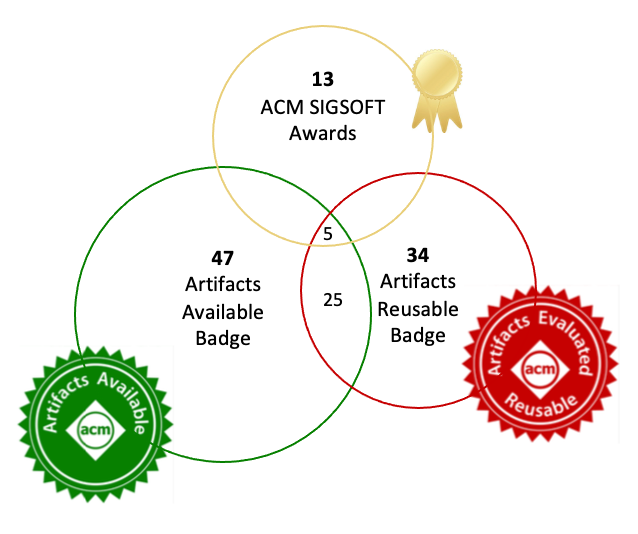
\includegraphics[clip,width=0.6\linewidth]{content/images/03-Awards}
    \caption{59 Publikationen mit Auszeichnungen}
    \label{img:awards}
\end{figure}

Zuerst werden die 13 Publikationen mit einer \textit{"ACM SIGSOFT"} Auszeichnung gelesen, danach die 25 Publikationen mit zwei Badges, die 21 Publikationen mit einem Badge und im Anschluss die restlichen Publikationen. Dabei ist die Reihenfolge innerhalb dieser vier Gruppe
abhängig von dem Vortragszeitpunkt auf der ICSE 2020 gewählt wurden, da dadurch die Publikationen bereits thematisch geclustert sind. \\
% TODO anders schreiben

Während dem erstmaligen Sichten einer Publikation, soll diese charakterisiert werden, welches eine weitere Aktivität des Vorgehens darstellt und in der Sektion \ref{sec:character} näher beschrieben wird.\\

Unter anderem wird abhängig von dieser Charakterisierung, aber auch abhängig von den in der 1. Iteration bereits identifizierten Kontexten und von den Themengebiet einer Publikation, die Publikationen gruppiert. Innerhalb dieser Gruppen werden die Publikationen in einer 2. Iteration erneut gesichtet und kritischer analysiert. \\



\section{Identifizierung von Kontextfaktoren}
Da der Aufwand eine Publikation komplett in voller Länger intensiv zu lesen nicht dem Nutzen alle Kontextfaktoren zu finden enspricht und angenommen wird das Kontextfaktoren unterschiedlich häufig an unterschiedlichen Stellen einer Publikation vorkommen, wird sich beim Sichten der Publikationen auf diese Stellen konzentriert. \\
Dazu wird im Folgenden weitere Annahmen getroffen zu den Stellen, an welchen Kontextfaktoren auftreten. \\

Es wird angenommen, dass Kontextfaktoren abhängig von dessen Zwecken an unterschiedlichen Stellen in einer konkreten Publikation vorkommen. \\
Denn Kontextfaktoren haben nicht nur den Zweck die Verallgemeinbarkeit einer Publikation zu beschreiben, wie in Kapitel 1 bei der Zielsetzung ausführlich erläutert, sondern auch zu anderen Zwecken. Denn es kann, wie bereits erwähnt, unterschieden werden zwischen den Kontext in den eine empirische Studie durchgeführt wurde und die Kontexte auf welche dessen Ergebnisse verallgemeinbar sind. \\
Dieser Zusammenhang zwischen dem Zweck eines Kontextfaktors und der Stelle in der Publikation wird im Weiteren erläutert und in der Tabelle \ref{table:vorkommen} aufgeführt. \\

In dem Titel und in der Einleitung einer Publikation ist zu erwarten, dass Kontextfaktoren zur Charakterisierung des Themenbereich oder zur Definition des untersuchten Problems verwendet werden. \\
Des Weiteren können Kontextfaktoren bei der Beschreibung einer Technik oder des Vorgehens einer empirischen Studie aufgeführt werden um Einzelheiten zu Beleuchten und zu Beschreiben in welchen Kontext Daten erhoben wurden. \\
Bei der Diskussion verwandter Arbeiten, haben Kontextfaktoren den Zweck die konkrete Publikation einzugrenzen und von anderen Publikationen abzugrenzen. An dieser Stelle können Kontextfaktoren genannt werden, die das Thema der Publikation einschränken und somit spezialisieren. Es kann beschrieben werden, in welchen Kontext die Studie nicht durchgeführt wurde und außerdem kann die Studie oder dessen Ergebnisse in Betrachtung anderer Arbeiten positioniert werden. \\
Bei den Schlussforgerungen, Nennung von Forschungsbeiträgen und bei der Diskussion zur Verallgemeinbarkeit wird unterem Anderem diskutiert, was die Validität der Publikation gefährden könnte und Kontextfaktoren diesbezüglich aufgestellt. Es ist zu Erwarten, dass an dieser Stelle viele Kontextfaktoren zu finden sind, die sich konkret auf die Verallgemeinbarkeit der Arbeit beziehen. \\

\begin{table}[h!]
\begin{tabular}{ r | l }
 Zweck & Vorkommen \\
  \hline
  Thema & Titel, Einleitung, Recherchefragen \\
  Detail & Beschreibung, Vorgehen, Datenerhebung \\
  Abgrenzung & Diskussion verwandter Arbeiten \\
  Verallgemeinbarkeit & Schlussfolgerungen, Forschungsbeiträge, Diskussion\\
\end{tabular}
\caption{Vorkommen von Kontextfaktoren nach Zweck}
\label{table:vorkommen}
\end{table}




Bei dem erstmaligen Sichten der Publikationen der ISCE 2020, wird sich auf die in Tabelle  \ref{table:vorkommen} aufgelisteten Stellen beschränkt. \\
Um sich einen Überblick über eine Publikation zu schaffen, werden zuerst die Titel der einzelnen Sektionen einer konkreten Publikation gelesen und zugeordnet, zu welchen Zweck Kontextfaktoren in einer konkreten Sektion vorkommen könnten. Anschließend werden die Sektionen, von denen vermutet wird, dass dort Kontextfaktoren vorkommen, in folgender Reihenfolge abhängig des Zweckes gelesen: Thema, Abgrenzung, Verallgemeinbarkeit. \\
Zunächst werden Sektionen, die sich auf das Thema der Publikation beziehen gelesen, um nicht nur Kontextfaktoren bezüglich des Themas zu finden, sondern auch um eine schnelle Einleitung in das Thema der Publikation zu erlangen. Anschließend werden die Sektionen bezüglich der Abgrenzung gesichtet, wie die Diskussion verwandter Arbeiten, um das Thema einzugrenzen. Danach werden die Sektionen bezüglich der Verallgemeinbarkeit, wie die Schlussfolgerungen und Diskussion gelesen. Dabei wird analysiert, welchen Beitrag die Publikation leistet. Erst in der 2. Iteration werden die Sektionen der Publikation angeschaut, die Details erläutern, und eine kritischere Analyse erfolgt.  \\

Bei dieser Lesetechnik, werden die Publikationen innerhalb zwei Iterationen nacheinander gesichtet. Das hat den Vorteil, dass es zu keinem Kontextwechsel kommt, wie es bei der Alternative der Fall wäre, wenn in vier Iterationen die Publikationen lediglich hinsichtlich eines Zweckes gesichtet werden, sprich zuerst werden alle Publikationen hinsichtlich des Themas gelesen, danach alle hinsichtlich der Verallgemeinerung, und so weiter. Dadurch könnte das Verständnis einer konkreten Publikation gemindert werden, sodass implizite Kontextfaktoren nicht entdeckt werden könnten. Jedoch hätte die Alternative den Vorteil, dass Beziehungen zwischen Kontextfaktoren verschiedener Publikationen bezüglich eines Zweckes besser erkannt werden könnten. \\

Da durch die Lesetechnik eventuell nicht alle Kontextfaktoren gefunden werden, wird in Kapitel \ref{chapter:evaluation} die Lesetechnik evaluiert und abgeschätzt, wie viele Kontextfaktoren unerkannt blieben als \textit{false negative}. Eine maximale bzw. vollständige Abdeckung ist jedoch nicht das Ziel dieser Arbeit. \\

Eine weitere Schwierigkeit ergibt sich dadurch, dass lediglich die Autorin dieser Masterarbeit alle Publikationen sichtet, Kontextfaktoren identifiziert und klassifiziert. Somit besteht zwar ein Grad an Einheitlichkeit. Jedoch könnten Verzerrungen und Bias entstehen. \\
Dies könnte verhindert werden, wenn mehrere Autoren und Autorinnen beteiligt wären und diese Aktivität unabhängig voneinander ohne gegenseitige Beeinflussung für eine zufällig ausgewählte Teilmenge der Publikation durchführen würden. Wenn sich dann noch die Teilmengen überschneiden, sodass jede Publikation mehrmals gesichtet wird, hat es den Vorteil, dass nicht nur mehr Kontextfaktoren identifiziert werden könnten, sondern auch, dass die interne Validität der Arbeit gestärkt wird. \\
Da jedoch nach der eidesstaatlichen Erklärung diese Arbeit komplett alleine durchgeführt wurde, ist dieser Ansatz nicht möglich. Allerdings wäre es vorstellbar, dass eine Folgearbeit geleistet werden kann, um Ergebnisse dieser Arbeit zu evaluieren und die interne Validität dieser Arbeit zu stärken. \\

Um die Qualität der Ergebnisse zu sichern, werden Argumentationsstränge so gut wie möglich offengelegt und es wird beschrieben,
wie aus den Textstellen konkreter Publikationen Schlussfolgerungen entstanden sind. Dadurch kann der Leser bzw. die Leserin dieser Masterarbeit sich eine eigene Meinung über die Ergebnisse bilden und die Argumentation verfolgen und bewerten. \\

\section{Klassifizierung von Kontextfaktoren}
\label{sec:class-context}
Im Anschluss der Sichtung einer konkreten Publikation werden die identifizierten Kontextfaktoren dieser Publikation klassifiziert und Faktorengruppen werden gebildet. Dabei wird ein Oberbegriff gefunden, der den Kontextfaktor beschreibt. Ein Beispiel dafür wäre, wenn eine Publikation \footnote{z.B. in der Publikation XXX} Softwareprojekte untersucht, die durch das Kriterium \textit{Nutzung von Java} ausgewählt wurden, lässt sich der Kontextfaktor \textit{Java} erkennen und ein passender Oberbegriff dafür, wäre \textit{Technologien}, welche die Faktorengruppe für alle Kontextfaktoren die Technologien beschreiben bildet. \\

Da bei den Publikationen die zuerst gesichtet werden, noch keine Klassen bzw. Faktorengruppen bestehen, weil die Faktorengruppen fortschreitend nach jeder Publikation ausgearbeitet werden, müssen die entstandenen Faktorengruppen und dessen zugeordneten Kontextfaktoren regelmäßig evaluiert und angepasst werden. Da alle Kontextfaktoren, die bereits zu einer Faktorengruppe zugeordnet sind, sich mit dem neuklassifizierten Kontextfaktor einer anderen Publikation ähneln müssen und die Faktorengruppe zu allen zugeordneten Kontextfaktoren passen muss. \\
Dabei kann es vorkommen, dass eine Faktorengruppe umbenannt wird auf einen mehr generalisierten Begriff, um alle Kontextfaktoren zu umfassen, oder dass eine Faktorengruppe auf zwei spezialisierte Faktorengruppen aufgeteilt wird, sodass eine Hierarchie von Faktorengruppen entstehen könnte. \\

%% TODO Lerneffekt EMPI \\

%% TODO \\
Wie bereits in Kapitel \ref{chapter:background} Sektion \ref{sec:verwandt} erwähnt, sollen ebenfalls verwandte Arbeiten evaluiert werden, um Kontextfaktoren und Faktorenklassen zu finden. Außerdem können geeignete Benennungen für Faktorengruppen  übernommen werden.


\section{Charakterisierung von Publikationen}
\label{sec:character}

Bei dem Leseprozess, sollen nicht nur Kontexte einer Publikation identifiziert werden. Die Publikation soll auch charakterisiert werden, damit Korrelationen zwischen Kontextfaktoren und den Publikationen erkannt werden können. \\

Im Gegensatz zu der Klassifizierung von Kontextfaktoren in Faktorengruppen, dessen Anzahl im Leseprozess steigt, werden die Charakterisierungskriterien und Optionen nicht fortschreitend auserarbeitend, sondern vorab definiert. \\
Da bereits in Kapitel \ref{chapter:background} \textit{Hintegrund} Sektion \ref{sec:empi} erläutert wurde, wie sich empirische Arbeiten unterscheiden können, wird hier nicht mehr näher dadrauf eingagen, sondern auf diese Sektion verwiesen. Anhand der Unterscheidungsfaktion von empirischer Arbeiten wurden Charakterisierungskriterien ausgewählt, welche in Kapitel \ref{chapter:background} \textit{Hintegrund} Sektion \ref{sec:empi} aufgelistet wurden. \\


\section{Dokumentierung und Erstellung von Artefakten}
Um diesen iterativen Prozess, welcher in Grafik \ref{img:process} dargestellt ist, zu bewerkstelligen und eine Übersicht von Kontextfaktoren und Faktorengruppen zu ermöglichen und eventuell bereits eine Hierarchie von Faktorengruppe abbilden zu können, werden die Werkzeuge \textit{MaxQDA} und \textit{Microsoft Excel} genutzt. \\

Mit Hilfe von \textit{MaxQDA} wurden die Publikationen gesichtet und markiert. Dabei wurden verschiedene Farben für verschiedene Zwecke genutzt.

\begin{itemize}
    \item rot für die Kontexte
    \item gelb für Notizen, Verständnis
    \item blau für Zitate bzgl der Verallgemeinbarkeit
    \item lila für Zitate bzgl Future Work oder Ergebnisse
    \item grün für die Charakterisierung der Publikation
\end{itemize}

Im Anschluss einer Sichtung wird mittels \textit{Microsoft Excel} die Publikation charakterisiert, und Kontext erfasst. Dabei werden Tabellen erstellt.

Es wurde sich für diese Werkzeuge entschieden, da diese für die Autorin kostenlos verfügbar sind.
Die entstandenen Artefakte sind im mx20.-Format und im xlsx.-Format zugänglich \footnote{Link zum github XX}.



%% TODO Verbindung um Kette von Kontextfaktoren innerhalb einer Publikation darzustellen? \\
%% TODO Kontextfaktor wird an vers Stellen der Publikation mehrmals erwähnt zu verschieden Zwecken und in vers Tiefe/Detailreiche/ Charakterisierung \\


\section{Analyse der Artefakte}
\label{sec:analysis-step}
Im nächsten Kapitel \ref{chapter:impl} \textit{Durchführung} wird nicht nur die bereits beschriebene Lesetechnik angewandet und das bereits erläuterte Vorgehen durchgeführt, sondern auch kritisch analysiert. Diese Analyse soll anhand folgender Recherchefragen geleitet werden, welche so wie das Vorgehen in Kapitel \ref{chapter:evaluation} \textit{Evaluation} evaluiert werden und somit beantwortet werden. \\

\paragraph{Recherchefrage 1:} Welche Kontextfaktoren werden in den Publikationen erwähnt? In wie weit beschreiben Autoren und Autorinnen den Kontext ihrer Publikationen? In welcher Form kommen Kontextfaktoren vor? Sind diese explizit oder implizit erkennbar? Sind andere Zwecke als, die in der Tabelle \ref{table:vorkommen} genannten, erkennbar?

\paragraph{Recherchefrage 2:} In wie weit diskutieren Autoren und Autorinnen über die Verallgemeinbarkeit ihr Publikationen, Ergebnisse und Techniken? Bestehen Lücken in den Diskussionen zur Verallgemeinbarkeit? Wie unterscheiden sich die Kontextfaktoren zum Zweck der Verallgemeinbarkeit zu den Kontextfaktoren anderer Zwecke?
%% TODO Threat of Validity, sollte viel drin stehen, aber oft nur Blabla \\

\paragraph{Recherchefrage 3:} Unterscheiden sich die Kontexte und Kontextfaktoren abhängig von den Arten der Publikationen und von der Vorgehensweise der empirischen Studie?

Bei der kritischen Analyse soll vor Allem die erstellten Artefakte genutzt werden, um relevante Daten für die Beantwortung der Recherchefragen sichtbar zu machen und auswerten zu können. Des Weiteren werden Korellationen und Zusammenhänge in geeigneten Grafiken visualisiert oder in Tabellen zusammengefasst.



%% TODO ISCE, Hohe Qualitaet, aber nicht immer relevant \\
%% TODO Bewertung der Existenzberechtigung eines Themas, starke/schwache Relevanzbegruendung? <-> Verallgemeinbarkeit \\

\section{Anfertigung einer Taxonomie}
Im Anschluss des bereits erläuterten Vorgehen werden ersten Schritte zu einer Taxonomie von Software Enginnering Kontexten gemacht. Dabei soll wie bei dem Schritt zur \textit{Analyse der Artefakten}, welcher in Sektion \ref{sec:analysis-step} dieses Kapitels erläutert wurde, das Datenbank Management System genutzt werden, wo bereits durch die Verbindungen zwischen Faktorengruppen eine Hierarchie erkennbar sein kann. \\
%% TODO überarbeiten

Jedoch besteht ein Kontext nicht nur aus einer Faktorengruppe, sondern aus mehreren. Daher soll analysiert werden, in welchen Kombinationen Faktorengruppe in den Publikationen vorkommen und in wie weit diese Kombinationen sich häufen. Dabei soll nicht nur der Kontext erkannt werden, in der eine empirische Arbeit durchgeführt wurde, sondern auch die Kontexte auf welche diese verallgemeinbar ist. \\
Wie bei dem Schritt zur \textit{Analyse der Artefakten}, welcher in Sektion \ref{sec:analysis-step} dieses Kapitels erläutert wurde, sollen geeignete SQL-Abfragen geschrieben werden, um die Kontexte aufzudecken.

Ebenfalls soll, wie im Schritt zur \textit{Klassifizierung von Kontextfaktoren}, welcher in Sektion \ref{sec:class-context} dieses Kapitels beschrieben wurde, verwandte Arbeiten genutzt werden, um die Kontexte und die Taxonomie zu evaluieren oder zu ergänzen.

%% TODO \section{} - Zusammenfassung, Beschreiben des Vorgehens \\
%% TODO Begriffe hinterfragen, zb. Commits, LoC – Gewicht? \\
%% TODO Öfteres Kodieren, semantische Konzepte sammeln \\



%%% Netzwerk zwischen Publikation -> durch Zurodnung von Kontexten?
%% Welche Publikation/Ergebnisse ist auf eine andere Publikation anwendbar/übertragbar?
%% Welche und wie viele Publikationen werden im gleichen Kontext geschrieben?

%% TODO Präsenz und Vergangenheitsformen abchecken - gehören Teile dieses Kapitels nicht eher in der Implementierung oder woanders hin? oder passen sie hier doch besser? Geschmacksache? \\

% Chapter 3
% - Gewählter Lösungsansatz, Alternativen, Abwägungen
